% Chapter 6

\chapter{Analysis and Discussion} % Main chapter title
\label{analysis}

\section{Per-Question Performance}

Table~\ref{tab:perq} and Figure~\ref{fig:perq} break ROUGE-L down by question. Each cell averages only 12 to 28 examples, so we read patterns across rows rather than individual cells.

\begin{table}[htbp]
    \centering
    \footnotesize
    \caption[ROUGE-L per question]{ROUGE-L per question on the test set (main protocol). Each cell averages 12--28 examples.}
    \label{tab:perq}
    \resizebox{\textwidth}{!}{%
    \begin{tabular}{lrrrrrrr}
        \toprule
        \tabinput{Tables/per_question_head.tex}
        \midrule
        \tabinput{Tables/per_question_body.tex}
        \bottomrule
    \end{tabular}}
\end{table}

\begin{figure}[htbp]
    \centering
    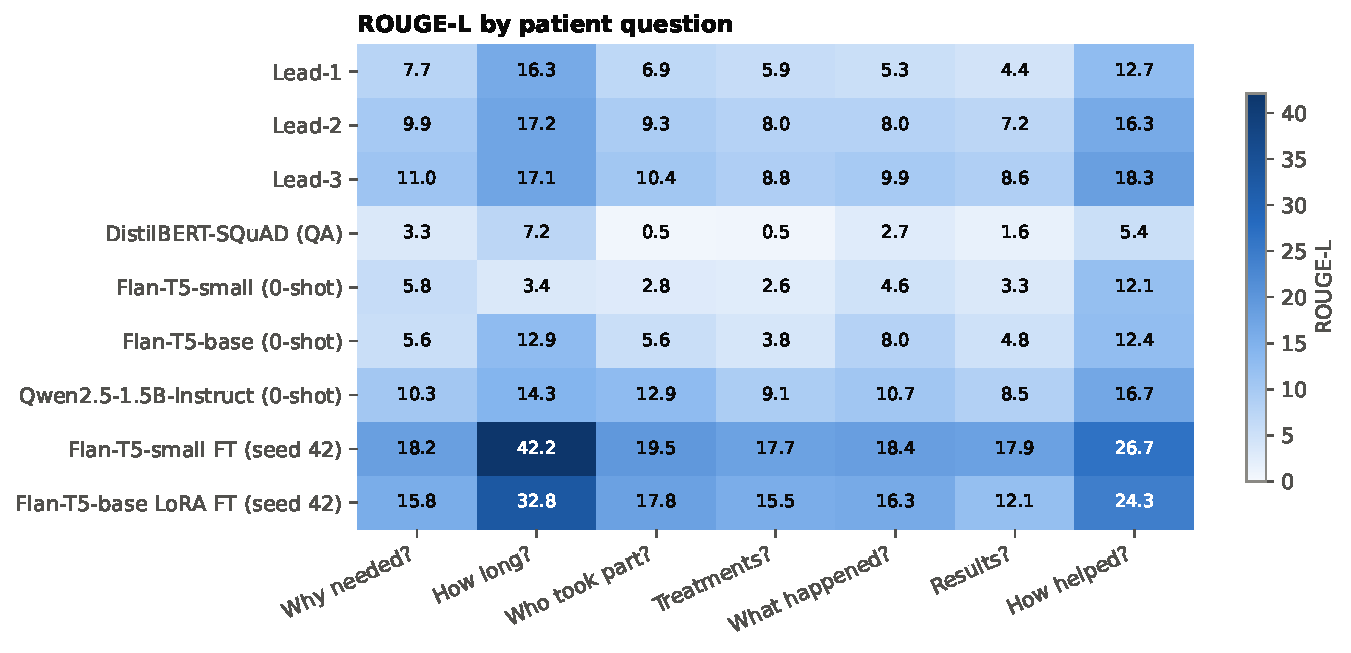
\includegraphics[width=\textwidth]{Figures/results/fig06_per_question_rougeL.pdf}
    \caption[ROUGE-L by question]{ROUGE-L by question.}
    \label{fig:perq}
\end{figure}

\emph{How long was the trial?} is the easiest question for the trained systems (fine-tuned Flan-T5-small: 42.2). Its answers are formulaic and the dates are present in the context. \emph{Results} and \emph{Treatments} are among the hardest for every system, which is consistent with the mapping defect described in Chapter~\ref{data}: these questions are answered only from the \emph{Conclusion} and \emph{Statistical Methods} sections respectively, so most of what the reference conveys is missing from the input. Fine-tuned Flan-T5-small has the highest ROUGE-L on all seven questions.

\section{Length and Readability of the Outputs}
\label{sec:length}

Table~\ref{tab:props} and Figure~\ref{fig:length} compare the outputs with the human references. Three groups emerge, and only the fine-tuned models resemble the references in both length and reading level.

\begin{table}[htbp]
    \centering
    \footnotesize
    \caption[Output properties]{Properties of the outputs on the test set (means; main protocol). FKGL: Flesch--Kincaid grade level. Novel bigrams: share of output bigrams absent from the context. Number and code support: share of numbers or drug/protocol codes in the output found in the context. Empty: share of empty outputs (\%).}
    \label{tab:props}
    \resizebox{\textwidth}{!}{%
    \begin{tabular}{lrrrrrrr}
        \toprule
        & Words & FKGL & Flesch & Novel bigrams & Number support & Code support & Empty \% \\
        \midrule
        \tabinput{Tables/output_properties_body.tex}
        \bottomrule
    \end{tabular}}
\end{table}

\begin{figure}[htbp]
    \centering
    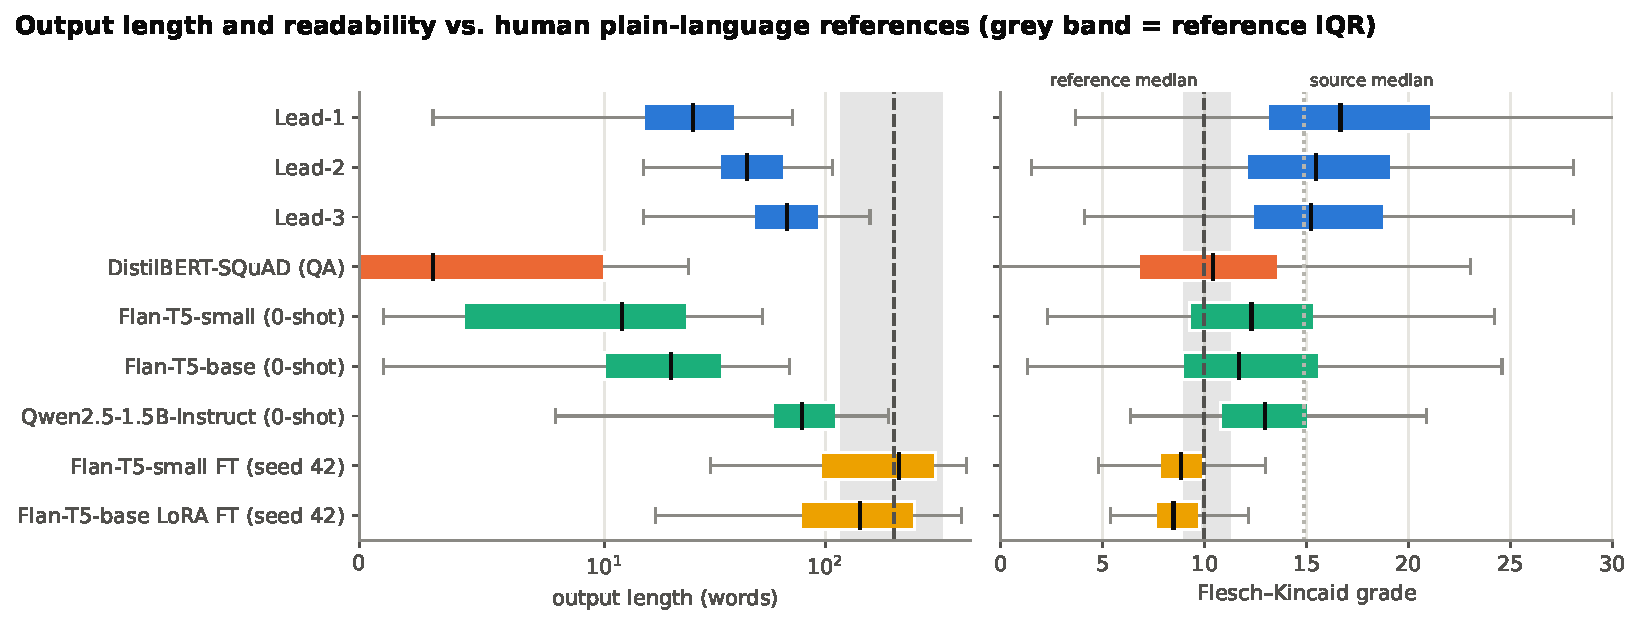
\includegraphics[width=\textwidth]{Figures/results/fig07_length_readability.pdf}
    \caption[Length and readability of outputs]{Output length and FKGL vs.\ the human references (grey band: reference interquartile range).}
    \label{fig:length}
\end{figure}

\begin{itemize}
    \item \textbf{Extractive systems} copy technical text and inherit its difficulty: Lead-3 has a mean FKGL of 17.57 and a Flesch score of 22.7.
    \item \textbf{Zero-shot generators are too short.} Zero-shot Flan-T5 outputs have a median of 12 (small) and 20 (base) words; Qwen's median is 78 words. Their FKGL (12.02 to 13.09) is lower than that of the source but higher than that of the references.
    \item \textbf{Fine-tuned models match the reference profile.} Fine-tuned Flan-T5-small has a mean FKGL of 9.28 against 10.27 for the human references, and a Flesch score of 57.8 against 54.9; LoRA is similar (9.24 and 58.2).
\end{itemize}

Fine-tuning therefore mainly teaches the \emph{register and length} of patient summaries. That alone accounts for part of the gain in overlap metrics, because length-matched outputs earn recall that short outputs cannot. The readability formulas measure only sentence and word length; a lower FKGL does not show that a text is good plain language, let alone that it is correct.

\section{Abstractiveness and Faithfulness Proxies}
\label{sec:faithfulness}

Figure~\ref{fig:faith} plots how much each system rewrites (novel bigrams) against the share of its numbers found in the source (number support). The ideal plain-language system would sit top right: it rewrites like the references without stating numbers the source does not support.

\begin{figure}[htbp]
    \centering
    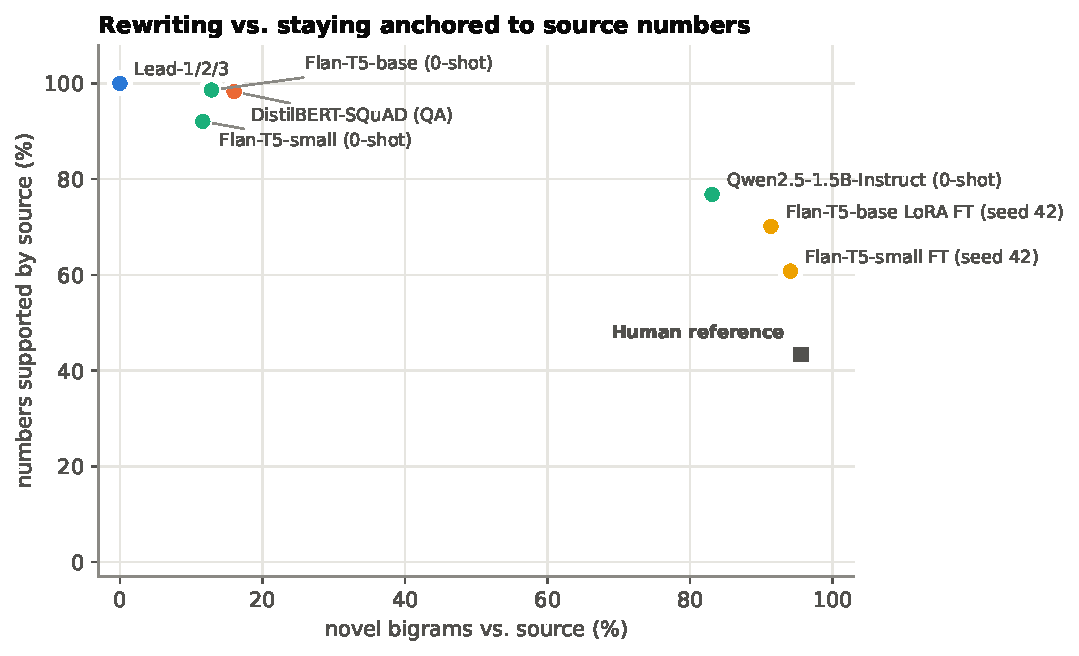
\includegraphics[width=0.85\textwidth]{Figures/results/fig08_abstractiveness_vs_faithfulness.pdf}
    \caption[Abstractiveness vs. number support]{Rewriting (novel bigrams) vs.\ numbers supported by the source. The grey square marks the human references.}
    \label{fig:faith}
\end{figure}

The horizontal axis separates copiers from rewriters. Lead-$k$, DistilBERT-SQuAD and zero-shot Flan-T5 rewrite little (novel-bigram shares of 0.00 to 0.16); Qwen (0.83) and the fine-tuned models (0.91 and 0.94) rewrite almost as much as the references (0.96).

The vertical axis needs care, because \textbf{the human references themselves have a number support of only 0.43 and a code support of 0.53}. Most numbers in a reference do not appear in its mapped context: the patient summaries draw on parts of the report that the question-to-section mapping does not provide. The input is under-specified for the target. The fine-tuned models sit between the copiers and the references, with number support of 0.61 (Flan-T5-small) and 0.70 (LoRA).

\emph{Interpretation.} Because the references contain details absent from the mapped input, models trained to imitate them are rewarded for producing such details. We read this as a property of the dataset construction, not only of the models, and we treat it as a moderate claim: it rests on a string-matching proxy, and the references are not ground truth for every fact. Number and code support do not measure factuality.

\section{A Typical Example}
\label{sec:example}

To illustrate what the scores hide, we inspect one test example: the question \emph{Why was the research needed?} for trial CAIN457H3301. It was chosen as the example whose fine-tuned Flan-T5-small ROUGE-L is closest to that model's median, so it is typical rather than selected for effect. Data licensing limits quotation to short fragments.

\begin{itemize}
    \item \textbf{Lead-3 and DistilBERT-SQuAD} copy the trial objective verbatim. This is accurate but not plain language.
    \item \textbf{Qwen} gives a correct but more technical paraphrase that keeps clinical jargon such as the BASDAI score (ROUGE-L 7.5, BERTScore $-$8.2).
    \item \textbf{Fine-tuned Flan-T5-small} reproduces the opening of the reference almost word for word (``Researchers are looking for a better way to treat\ldots''), then degrades into garbled terms such as ``sapondyritis'' and a misspelt drug name, ``scukinumab''. It has the highest ROUGE-L of all systems on this example (19.5) and the second-highest BERTScore ($-$5.4).
    \item \textbf{Flan-T5-base with LoRA} has the highest BERTScore on the example ($-$1.9) but introduces conditions the source does not mention, such as an ``active bladder infection'' and a drug ``used to treat septicemia''.
\end{itemize}

On this example the automatic metrics rank the outputs by stylistic similarity to the reference, not by correctness; the output a patient could most safely read comes from the zero-shot Qwen model, which scores lower on both metrics.

\section{Why Extractive Question Answering Does Not Fit}
\label{sec:extractive}

No reference occurs verbatim in its source section (Section~\ref{sec:targets}), so span-extraction labels are undefined for every example. In the original pipeline, span labels were computed by searching for the answer string in the context; this search fails for all 959 examples, and every training label collapses to the ``no answer'' position. Empirically, the off-the-shelf DistilBERT-SQuAD model is the weakest system in the study (ROUGE-L 2.72) and returns an empty answer for 40.6\% of the test examples. The task is abstractive by construction, and an extractive model cannot in principle reproduce its targets.

\section{Answers to the Research Questions}

\paragraph{RQ1: Can small CPU-trainable models match human summaries better than the baselines?} By every automatic metric, yes. Fine-tuned Flan-T5-small reaches a ROUGE-L of 22.36 $\pm$ 0.39 over three seeds, roughly double that of Lead-3 (11.41), with non-overlapping confidence intervals and Holm-corrected paired tests, and it matches the references in length and readability (FKGL 9.28 against 10.27). Each fine-tuning run took about one and a half hours on a CPU. This answer concerns similarity to the references, not correctness (RQ4).

\paragraph{RQ2: Does the extractive QA framing suit the task?} No. No reference is a substring of its context, so span labels are undefined, and the extractive model is the weakest system.

\paragraph{RQ3: How sensitive are the conclusions to decoding and metric choice?} Highly. Under plain greedy decoding, ROUGE ranks a model that loops in 86\% of its outputs above Lead-3, while BERTScore ranks it below every system in the main table. Under the main protocol, Qwen ties Lead-3 on ROUGE-L but is clearly ahead on BERTScore.

\paragraph{RQ4: Do automatic metrics reflect faithfulness?} The evidence so far suggests not. Qualitative inspection and string-level faithfulness proxies suggest that the automatic metrics reward the style of patient summaries more than their correctness: the systems that win every metric produce garbled or unsupported content on a typical example, and the references themselves contain many numbers and codes absent from the input. This claim is of moderate strength. It rests on proxies and one systematically chosen example; the planned human evaluation (Section~\ref{sec:limitations}) is needed to confirm or reject it.

No system in this study produces summaries that can be considered factually reliable or safe for patients without human review.
